\begin{figure}[t!]
  \centering
  \begin{subfigure}{1.0\textwidth}
    \centering
    \footnotesize
    \begin{tikzpicture}[xscale=0.9,yscale=0.4]
      % LFSR interactions
      \draw (0, -0.5) rectangle (3, 0.5) node[pos=0.5]{$\pseudoKS$ {\tiny \emph{(Key schedule)}}} ;
      \draw (0, 2.5) rectangle (3, 3.5) node[pos=0.5]{$\whitening$ {\tiny \emph{(whitening LFSR)}}} ;
      \draw (4, 0) node[inner sep=0pt](addm){$\boxplus$} ;
      \draw[->] (3, 0) -- (addm) ;
      \draw[->] (3.5, 0) -- (3.5, 1) -- (1.5, 1) -- (1.5, 0.5) ;
      \draw[->] (3.5, 3) -- (3.5, 4) -- (1.5, 4) -- (1.5, 3.5) ;
      % FSM
      \draw[color=white] (5, -0.5) rectangle (6, 0.5) node[pos=0.5,color=black]{$\subW$} ;
      \draw[color=white] (8, -0.5) rectangle (9, 0.5) node[pos=0.5,color=black]{$\shiftR$} ;
      \draw[color=white] (10, -0.5) rectangle (11, 0.5) node[pos=0.5,color=black]{$\mixC$} ;
      \draw (6, -2.5) rectangle (8, -1.5) node[pos=0.5]{FSM state};
      \draw[->] (addm) -- (5, 0) ;
      \draw[->] (6,0) -- (8, 0) ;
      \draw[->] (9,0) -- (10, 0) ;
      \draw[->] (11,0) -- (11.5, 0) -- (11.5, -2) -- (8, -2);
      \draw[->] (6, -2) -- (4, -2) -- (addm) ;
      % extracting
      \draw[color=white] (6.5, 1) rectangle (7.5, 2) node[pos=0.5,color=black]{$\filter$} ;
      \draw(7, 3) node[inner sep=0pt](addr){$\boxplus$};
      \draw (10, 3) node(s){$Z_t$} ;
      \draw[->] (3, 3) -- (addr) ;
      \draw[->] (7, 0) -- (7, 1) ;
      \draw[->] (7, 2) -- (addr) ;
      \draw[->] (addr) -- (s) ;
      % wire width
      \draw (4.45, -0.2) -- (4.55, 0.2) ;
      \draw (4.5, 0.5) node{$16$} ;
      \draw(4.45, 2.8) -- (4.55, 3.2) ;
      \draw (4.5, 3.5) node{$4$} ;
    \end{tikzpicture}
    \caption{\label{fig:diagram}General structure (rectangles correspond to registers).}
  \end{subfigure}
  \vspace{1em}

  \hfill
  \begin{subfigure}{0.2\textwidth}
    \centering
    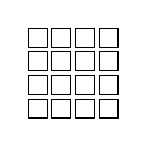
\begin{tikzpicture}[xscale=0.3,yscale=0.3]
      \tiny
      \foreach \i in {0,...,3}{
        \foreach \j in {0,...,3}{
          \draw (\i+0.1, \j+0.1) rectangle (\i+0.9,\j+0.9) node[pos=0.5]{$\thesbox$} ;
        }
      }
    \end{tikzpicture}
    \caption{\label{fig:SW}$\subW$.}
  \end{subfigure}
  \hfill
  \begin{subfigure}{0.2\textwidth}
    \centering
    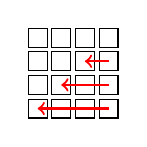
\begin{tikzpicture}[xscale=0.3,yscale=0.3]
      \tiny
      \foreach \i in {0,...,3}{
        \foreach \j in {0,...,3}{
          \draw (\i+0.1, \j+0.1) rectangle (\i+0.9,\j+0.9) ;
        }
      }
      \draw[color=red,style=thick,->] (3.5, 0.5) -- (0.5, 0.5) ;
      \draw[color=red,style=thick,->] (3.5, 1.5) -- (1.5, 1.5) ;
      \draw[color=red,style=thick,->] (3.5, 2.5) -- (2.5, 2.5) ;
    \end{tikzpicture}
    \caption{\label{fig:SR}$\shiftR$.}
  \end{subfigure}
  \hfill
  \begin{subfigure}{0.2\textwidth}
    \centering
    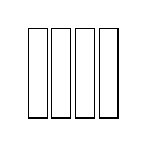
\begin{tikzpicture}[xscale=0.3,yscale=0.3]
      \tiny
      \foreach \i in {0,...,3}{
          \draw (\i+0.1, 0.1) rectangle (\i+0.9,3.9) node[pos=0.5]{$\mixmat$} ;
      }
    \end{tikzpicture}
    \caption{\label{fig:MC}$\mixC$.}
  \end{subfigure}
  \hfill
  \begin{subfigure}{0.25\textwidth}
    \centering
    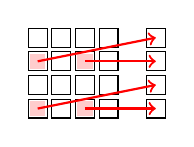
\begin{tikzpicture}[xscale=0.3,yscale=0.3]
      \footnotesize
      % state grid and output
      \foreach \i in {0,...,3}{
        \foreach \j in {0,...,3}{
          \draw (\i+0.1, \j+0.1) rectangle (\i+0.9,\j+0.9) ;
        }
        \draw (5.1, \i+0.1) rectangle (5.9, \i+0.9) ;
      }
      % colored squares
      \draw[color=white, fill=red!20] (0.15, 0.15) rectangle (0.85, 0.85) ;
      \draw[color=white, fill=red!20] (2.15, 0.15) rectangle (2.85, 0.85) ;
      \draw[color=white, fill=red!20] (0.15, 2.15) rectangle (0.85, 2.85) ;
      \draw[color=white, fill=red!20] (2.15, 2.15) rectangle (2.85, 2.85) ;
      % arrows
      \draw[color=red,style=thick,->] (0.5, 0.5) -- (5.5, 1.5) ;
      \draw[color=red,style=thick,->] (2.5, 0.5) -- (5.5, 0.5) ;
      \draw[color=red,style=thick,->] (0.5, 2.5) -- (5.5, 3.5) ;
      \draw[color=red,style=thick,->] (2.5, 2.5) -- (5.5, 2.5) ;
    \end{tikzpicture}
    \caption{\label{fig:filter}$\filter$.}
  \end{subfigure}
  \hfill~
  
  \caption{\label{fig:structure}A high level view of \coolName.}
\end{figure}


% Leo: ce qui suit est pour qu'emacs compile bien l'article, pas touche !
%%% Local Variables:
%%% mode: latex
%%% ispell-local-dictionary: "english"
%%% TeX-master: "../main"
%%% End:



